%\documentclass[12pt]{article}
\documentclass[journal]{IEEEtran}
\usepackage[utf8]{inputenc}
\usepackage{listings}
\usepackage{lipsum}
\usepackage{graphicx}
\usepackage[spanish]{babel}
\usepackage{tikz}
\usepackage{pgf-pie}
\usepackage{babel,blindtext}
\usepackage{color}



% Custom colors
\definecolor{deepblue}{rgb}{0,0,0.5}
\definecolor{deepred}{rgb}{0.6,0,0}
\definecolor{deepgreen}{rgb}{0,0.5,0}

% Default fixed font does not support bold face
\DeclareFixedFont{\ttb}{T1}{txtt}{bx}{n}{07} % for bold
\DeclareFixedFont{\ttm}{T1}{txtt}{m}{n}{06}  % for normal

\lstdefinestyle{python_gabo}{
  breaklines=true,
	language=Python,
	basicstyle=\ttm,
	otherkeywords={self},             % Add keywords here
	keywordstyle=\ttb\color{deepblue},
	emph={MyClass,__init__},          % Custom highlighting
	emphstyle=\ttb\color{deepred},    % Custom highlighting style
	stringstyle=\color{deepgreen},
	frame=tb,                         % Any extra options here
	showstringspaces=false,            % 
  commentstyle=\ttb,
}


\begin{document}

\title{Trabajo Práctico Final de Reglas de Asociacion}
\author{
	Keuroghlanian, Alejo \\
	\and
	Krauthamer, Diego \\
	\and
	Moncarz, Gabriel}
\maketitle % this produces the title block

\begin{abstract}
Trabajo de investigación de Reglas de Asociación con perfil académico. Se desarrollan
todos los pasos que deben seguirse para la construcción de reglas de asociación
y su posterior análisis. Las reglas son procesadas mediante el algoritmo Apriori.
El trabajo se desarrolla en conjunto con  un ejemplo
práctico, donde se analizan personas que califican películas. El objetivo es encontrar 
características que definan a los usuarios, a las películas y a sus
relaciones conjuntas. 

El procesamiento se ha realizado con los software
Weka y R, mostrando R un rendimiento
adecuado para la complejidad computacional del problema.

Finalmente se muestran en detalle todos los patrones encontrados, siendo el más 
relevante que el estado de California y Minnesota son outliers.
\end{abstract}

\begin{IEEEkeywords}
Reglas de asociación
Apriori
Minería de datos
Aprendizaje automática
Películas
\end{IEEEkeywords}







\section{Introducción}

Las reglas de asociación son una herramienta de aprendizaje automático para
tratar de identificar patrones comunes no triviales en conjuntos de datos
extensos. La idea general es hacer un análisis exploratorio para  encontrar 
asociaciones del estilo \{A\} $=$$>$ \{B\}, que significan 
``si sucede A, entonces sucede B''. 

El trabajo presentado se orienta a hacer un análisis de reglas de asociación con
fines académicos. Se pretender explorar como funcionan, cuales son  su desempeño y
cuales son el tipo de asociaciones que se pueden generar. Para esto se
hace un análisis en profundidad de un problema en particular. Se
explica en detalle cada uno de los pasos realizados y se justifica cada una de 
las decisiones tomadas.

El problema a desarrollar esta relacionado con la industria cinematográfica.
Se tiene información de usuarios que califican películas. Se pretende encontrar
las preferencias de los usuarios, sus gustos, sus características según su
posición demográfica y si ha habido algún cambio de tendencia en las valuaciones
con del transcurso del tiempo.

En la sección de Datos se detalla los datos fuentes, como se los transforma,
discretiza y preprocesa para generar información útil y cómoda para un análisis
de reglas de asociaciones; En la sección de Procesamiento de datos se 
explica los software utilizados, ventajas y defectos, como la elección de los
parámetros idóneos de los algoritmos; En la sección de Análisis se interpretan
las reglas de asociaciones obtenidas; En la sección de Conclusiones se enuncian
las conclusiones del trabajo; Y por último, se enuncian las posibles mejoras
que pueden realizarse como algunos comentarios finales.



\section{Datos}
En la presente sección se analiza los datos originales, como fueron enriquecidos,
como se los ha manipulado y las transformaciones realizadas. También se explica como 
el procesamiento se ha automatizado 
de forma íntegra, con intenciones de que este mismo análisis 
pueda realizarse en caso de tener datasets distintos, como si se desease incorporar
nuevas entradas a los datos existentes.

\subsection{Fuente de datos}
El punto de partida del presente trabajo son  archivos relacionados con información
sobre pelícuas y rating de películas. Los archivos en cuestión son 3:
\begin{enumerate}
	\item Peliculas: contiene 3.883 películas a ser analizadas. La información sobre cada
		una de ellas es:
		\begin{itemize}
			\item Código de película
			\item Nombre de la película
			\item Lista de géneros a la que pertenece
				\begin{lstlisting}[frame=single, breaklines=true]
1::Toy Story (1995)::Animation|Children's|Comedy
2::Jumanji (1995)::Adventure|Children's|Fantasy
3::Grumpier Old Men (1995)::Comedy|Romance
4::Waiting to Exhale (1995)::Comedy|Drama
5::Father of the Bride Part II  (1995)::Comedy
				\end{lstlisting}
		\end{itemize}


	\item Usuarios: contiene 6.040 registros de usuarios distintos. La información de cada
		fila es
		\begin{itemize}
			\item código de usuario
			\item sexo (masculino o femenino)
			\item rango de edad
			\item ocupación o profesión
			\item código postal del usuario\footnote{Todos los usuarios analizados residen 
			  en los Estados Unidos}
				\begin{lstlisting}[frame=single]
1::F::1::10::48067
2::M::56::16::70072
3::M::25::15::55117
4::M::45::7::02460
5::M::25::20::55455
				\end{lstlisting}
		\end{itemize}

	\item Rating: rating de distintos usuarios sobre diversas películas.\footnote{Se
		destaca que cada usuario emite la calificación sobre las películas que él desea. El
		usuario no está obligado a completar una cantidad mínima de calificaciones.}

		\begin{itemize}
			\item Usuario que realiza la evaluación
			\item Pelicula evaluada
			\item Rating/evaluación asignada
			\item tiempo: momento en que es evaluada

        \begin{lstlisting}[frame=single,breaklines=true]
1::1193::5::978300760
1::661::3::978302109
2::3108::3::978299712
2::3035::4::978298625
5::3081::3::978243054
5::377::4::978245999
        \end{lstlisting}
    \end{itemize}

\end{enumerate}

Estos 3 archivos son, en resumen, los datos crudos utilizados. 
Todo el tratamiento de datos posterior, tanto el enriquecimiento de información como los
análisis y conclusiones finales, están basados en el contenido de estos 3 archivos
fuentes.

\subsection{Automatización para el preprocesamiento}
El objetivo de la automatización de los datos es generar un algoritmo que se encargue
de hacer todo el preprocesamiento de la información. Las tareas del preprocesamiento
son: eliminación  y tratamiento  de datos faltantes o erroneos, filtrado de información,
agrupamiento y/o transformación.
\emph{El objetivo principal de este proceso es que su salida genere información clara, limpia y cómoda
para ser procesada por los algorítmos de análisis propiamente dicho -Apriori en este caso-.}

Lo primero que se hace es conocer los datos de forma general, hacer un análisis descriptivo,
exploratorio, conocer que tipo de datos son, sus frecuencias y relaciones. Luego se realiza un
borrador de los procesos que se debe correr a los datos para generar la información de salida 
deseada. El mayor inconveniente es que \emph{no siempre se conoce de antemano cuales son las
salidas ideales a generar}. Es frecuente una vez que se está haciendo el análisis profundo
de los datos, creer conveniente tener los datos en distintos formatos, estructuras de
datos u ordenes de los generados. Muchas veces, cambiar estos archivos de salida no 
es sencillo, o demanda tiempo.

Existen varias alternativas para resolver este inconveniente de raíz
. La realizada en el presente
trabajo es desarrollar un software cuyas entradas sean los 3 archivos presentados en 
la sección de datos. Estos archivos son procesados automáticamente, pero el usuario
puede implementar diferentes funciones de salida ad-hoc, que determinan cuales son
las salidas a generar, formatos, ordenes, etc.

Existen ocasiones en los que el usuario encuentra un formato eficiente, pero la cantidad
de datos generados es mayor a la necesaria, haciendo que el proceso de análisis posterior corra
mas lento de lo necesario. Por ejemplo, si se quiere analizar géneros de películas y
estados demográficos, tener un set de datos con actores y profesiones de los calificadores
es irrelevante, consume más memoria, demanda mas tiempo en procesar datos innecesarios
y podría llegar a hacer que el análisis sea abortado.

Es para solucionar este tipo de inconvenientes que el desarrollo realizado hace un
procesamiento inicial de los datos, los limpia y transforma tanto como puede, y luego
deja para el usuario escoger filtros y procesamientos ad-hoc para su salida final.

En caso que el usuario, durante el análisis de reglas de asociación, crea conveniente
tener un nuevo set de datos con otras características, sólo debe implementar su
nueva función de salida (generalmente se modifican parámetros de las funciones ya
existentes), para luego correr el algoritmo y tener la información lista para ser 
procesada.
La lista \ref{code:pre_process_output} muestra uno de los generadores de salida
usados en el trabajo.

\begin{lstlisting}[style=python_gabo,
	caption={Descriptive Caption Text} ,label=code:pre_process_output,
	]
def writeTransActorsDirectors(filename, moviesDict, usersDict, ranking="high",
  writeGenre=False, ratingYear=None):
    """Write a transaction file ready to be process by R.

    The function is able to generate a basic output structure with optionales
    fields. 
    The parameters are:
     * filename: output filename 
     * moviesDict: dictionary of moviews
     * usersDict: Dictionary with the users that calified movies
     * ranking: only display the transaction whose quialification is equal to
        this parameter. If ranking=None, the filter will write all transactions
     * writeGenre: Choose to write the movies genres
     * ratingYear: list that filter only the years that the rating were performed
    """
    CSV_CHAR = ','
    # Open the File
    try:
        fh = open(filename, 'w')
    except:
        return None

    # Write the header
    header = ['tid', 'pid']
    line = CSV_CHAR.join(header)
    fh.write(line.encode('utf-8'))
    fh.write('\n')

    transid = 0
    for movie in moviesDict.values():
        if movie.rating and movie.imdbRating:
            cast = map((lambda x: "actor_" + x), movie.cast) if movie.cast else ['?']
            genres = movie.genre if movie.genre else ['?']

            if movie.director:
                fixedMovie = [movie.name, "director_" + movie.director ]
            else:
                fixedMovie = [movie.name]

            for rating in movie.rating:
                if ranking == None or rating.ratingCat == ranking:
                    currentRatingYear = int(datetime.datetime.fromtimestamp(int(rating.timestamp)).strftime('%Y'))
                    if ratingYear==None or currentRatingYear in ratingYear:
                        transid += 1
                        user = usersDict[rating.userid]
                        fixedUser = [user.ageCat, "prof_" + user.profession]
                        fixedRating = [ rating.ratingCat ]

                        lst = fixedMovie[:]
                        lst.extend(fixedUser)
                        if ranking == None:
                            lst.extend(fixedRating)
                        lst.extend(cast)
                        if writeGenre:
                            lst.extend(map((lambda x: "genre_" + x), genres))
                        lst = map(unicode, lst)
                        for item in lst:
                            fh.write(('%d,"%s"\n' %(transid, item)).encode('utf-8'))

    h.close()
\end{lstlisting}


\subsection{Software de automatizacion}
El desarrollo para la automatización de preprocesamiento es realizado por 
los integrantes del trabajo en Python, bajo licencia GNU. Se lo puede bajar,
usar y clonar\footnote{El término adecuado es fork}. Esta alojado en GitHub, en la 
dirección https://github.com/gmoncarz/movie-asoc-rules. 

El work-flow\footnote{Flujo de trabajo en castellano} del software a nivel conceptual es:
\begin{enumerate}
\item Leer un archivo de configuración. Este archivo 
contiene los archivos de entrada y los de salida,
como también parámetros generales del algoritmo.
El usuario, si lo desea, puede generar sus parámetros custom. De
esta forma, la configuración del preprocesamiento esta cargada en este
archivo. El usuario tiene la posibilidad de generarse varios archivos
de configuración, de acuerdo a las salidas deseadas.
\item Cargar las películas del archivo de entrada.
\item Leer información adicional de cada película.
\item Preprocesar las películas de forma aislada.
\item Cargar los usuarios del archivo de entrada.
\item Leer información adicional de los usuarios.
\item Preprocesas los usuarios.
\item Leer los ratings del archivo de entrada.
\item Asociar las películas y los usuarios a través de los ratings.
\item Generar los archivos de salida.
\end{enumerate}

Es importante aclarar que este desarrollo, desde sus comienzos,
es diseñado para trabajar con grandes cantidades de datos con relativa
eficiencia. Pese a que hay unos cuantos detalles de performance 
y estilo por pulir,
los datos \textbf{no} están cargados todos en memoria. Se usan estructuras
de datos con persistencia. Esto significa que los datos son cargados en
archivos binarios, eficientes, y se va accediendo a ellos mediante
un cache en memoria. De esta manera, la cantidad de datos a preprocesar
no se encuentra limitada por la memoria de la computadora donde
el software se ejecuta.

\subsection{Discretización y transformación de datos}
Una vez que las instancias se cargan, se hace una limpieza básica de datos.
Ésta consiste en verificar la existencia de datos, que éstos pertenezcan
al dominio de datos (ie. películas no vacías, años luego de 1900 e inferiores
al año actual, que el sexo de los usuarios sean masculino o femenino, que las
profesiones estén en el rango definido, etc.)

El segundo paso consiste hacer algunas transformaciones de datos. Los nombres
de películas aparecen junto al año de creación entre paréntesis. Esos campos se 
separan y se almacenan de forma independiente. A los códigos se les
asigna una descripción para que los objetos, en etapa de debuging, 
puedan ser representados e identificados con facilidad. Por ejemplo, a la profesión 2 se 
le asigna ``academic / teacher'', a la edad cuyo código es 24, se le asigna
una descripción ``18-24''.

Por último se hacen algunas discretizaciones de datos. A los años en que
las películas fueron lanzadas se los discretiza según la década de creación
 (por ejemplo, 1993 $-$$>$ 1900; 2002 $-$$>$ 2000, etc). 
También se discretizan los rating de calificaciones. Las calificaciones de
1 y 2 pasan a tener la categoría baja; la de 3 como categoría media; y las
calificaciones 4 y 5 como categoría alta. 

Todas las transformaciones y discretizaciones utilizadas pueden ser modificadas
por el usuario según el criterio que crea conveniente. 



\subsection{Obtención de datos externos}
Con el objetivo de enriquecer los datos existentes y generar reglas de asociación
no triviales, se obtienen de terceras partes datos adicionales.

Por un lado se obtienen los directores y actores de las películas cargadas. Esta información se
obtiene de la base de datos de IMDB\footnote{Ver www.imdb.com}. Como cada película puede
tener más de un actor y un director, el software no va a cargar todos, sino los más importantes
de cada campo. Esta cantidad esta predefinida para que retorne el mejor director y los 
5 mejores actores. Sin embargo, estos valores pueden ser modificados por el usuario.

Uno de los mayores inconvenientes al obtener datos externos es la latencia. Para tener
los actores de IMDB se necesita hacer al menos 2 requests HTML. Uno es para buscar la
película en base al nombre. Esta consulta devuelve una lista de películas o series con
las búsquedas que más se asemejan al string de entrada. El segundo request es para 
escoger información específica de la película (actores y directores en este caso), una vez
que se conoce el código de película según la salida del primer request.

Estos 2 requests pueden llegar a demorar unos 20 a 30 segundos por película. Si el archivo de
entrada tiene 3950 películas, el proceso demanda aproximadamente 22 hs por corrida.

Este tiempo puede ser mejorado, pero la eficiencia de ese proceso esta fuera del alcance del trabajo.
Lo que no queda fuera de alcance, es la restricción de que cada vez que el usuario desea
generar un nuevo set de datos con alguna variación respecto al anterior, éste debe esperar
22 hs para obtener su nueva salida. Es para evitar este percance que se implementa un cache interno, 
eficiente y serializado, que almacena los datos de IMDB de las películas ya accedidas previamente.
Esto implica que cuando se carga una película, el software busca si ya la tiene en su cache,
 si la tiene, usa esa información. Si no a tiene, la busca en IMDB y la almacena, para que 
pueda accederse en la iteración siguiente. De este modo, las 22 hs de espera se reducen a
unos milisegundos para cargar la estructura de datos del cache serializado.

Por otro lado, se ha cruzado la información del código postal de cada usuario, para
obtener la ciudad y el estado de residencia, con intenciones de intentar descubrir
si hay asociaciones demográficas.

\subsection{Generación de datasets}
Durante el desarrollo del trabajo se ha generado, en total, mas de 20 datasets y 4 GB de datos descomprimidos. 
Las diferencias entre estos radican en el formato utilizado, cantidad de datos y atributos. Estas variantes se
usan para conocer en profundidad los software que operan con reglas de asociaciones, y
ver cual es el impacto en tiempo de procesamiento y memorial, al agregarles mas
datos y atributos.
También se ha probado la performance bajo diferentes formatos de dataset.

\begin{lstlisting}[frame=single,breaklines=true]

# Formato que repite en cada fila los campos fijos, pero altera los campos variables 

1|Toy Story|1995|John Lasseter|8.3|Tom Hanks|Animation|3737|male|56-inf|retired|Murfreesboro|TN|4|2000
1|Toy Story|1995|John Lasseter|8.3|Tom Hanks|Animation|1004|male|56-inf|Artist|San Jose|CA|5|2000
1|Toy Story|1995|John Lasseter|8.3|Tom Hanks|Animation|550|male|56-inf|executive|NA-citi|NA-state|5|2000
1|Toy Story|1995|John Lasseter|8.3|Tom Hanks|Animation|5301|male|56-inf|independent|Vega Baja|PR|5|2000
1|Toy Story|1995|John Lasseter|8.3|Tom Hanks|Animation|5827|male|56-inf|academic / teacher|Saint Paul|MN|4|2000
1|Toy Story|1995|John Lasseter|8.3|Tom Hanks|Animation|1248|female|56-inf|unemployer|Walnut Creek|CA|2|2000
1|Toy Story|1995|John Lasseter|8.3|Tom Hanks|Animation|2071|male|56-inf|doctor / health care|Worcester|MA|4|2000
1|Toy Story|1995|John Lasseter|8.3|Tom Hanks|Animation|1978|male|56-inf|housewife|West Liberty|OH|3|2001
1|Toy Story|1995|John Lasseter|8.3|Tom Hanks|Animation|4715|male|56-inf|academic / teacher|Portland|OR|5|2000
1|Toy Story|1995|John Lasseter|8.3|Tom Hanks|Animation|2848|male|56-inf|unknown|Bloomington|IN|5|2000


# Formato similar al 1ero, pero los datos fijos los escribe en la primer fila
# y en las filas subsiguientes los escribe como datos faltantes
tid,name,year,director,actor,genre,uid,sex,ageCat,prefession,citi,state,rating
1,"Prince of the City","1980","Sidney Lumet",?,?,"2503","male","35-44","independent","New London","PA","low"
1,?,?,?,"Treat Williams",?,?,?,?,?,?,?,?
1,?,?,?,"Jerry Orbach",?,?,?,?,?,?,?,?
1,?,?,?,"Richard Foronjy",?,?,?,?,?,?,?,?
1,?,?,?,"Don Billett",?,?,?,?,?,?,?,?
1,?,?,?,"Kenny Marino",?,?,?,?,?,?,?,?
1,?,?,?,?,"Drama",?,?,?,?,?,?,?
2,"Prince of the City","1980","Sidney Lumet",?,?,"2857","male","25-34","unknown","Bronx","NY","medium"
2,?,?,?,"Treat Williams",?,?,?,?,?,?,?,?
2,?,?,?,"Jerry Orbach",?,?,?,?,?,?,?,?
2,?,?,?,"Richard Foronjy",?,?,?,?,?,?,?,?
2,?,?,?,"Don Billett",?,?,?,?,?,?,?,?
2,?,?,?,"Kenny Marino",?,?,?,?,?,?,?,?
2,?,?,?,?,"Drama",?,?,?,?,?,?,?

# Formato de transacciones. El primer campo es el transactionID y en el 
# segundo se tiene el product id.
tid,pid
1,"Prince of the City"
1,"director_Sidney Lumet"
1,"25-34"
1,"prof_doctor / health care"
1,"Columbus"
1,"OH"
1,"male"
1,"high"
1,"actor_Treat Williams"
1,"actor_Jerry Orbach"
1,"actor_Richard Foronjy"
1,"actor_Don Billett"
1,"actor_Kenny Marino"
1,"genre_Drama"
2,"Prince of the City"
2,"director_Sidney Lumet"
2,"50-55"
2,"prof_other"
2,"Columbia"
2,"MO"
2,"female"
2,"medium"
2,"actor_Treat Williams"
2,"actor_Jerry Orbach"
2,"actor_Richard Foronjy"
2,"actor_Don Billett"
2,"actor_Kenny Marino"
2,"genre_Drama"

\end{lstlisting}

Es importante remarcar que estos datasets se generan dinámicamente, de forma 
no supervisada. El usuario solo requiere bajar el software de GitHub, instalar
las librerías básicas y correr el software, indicando el archivo de configuración
\footnote{En github se encuentra el archivo de configuración ejemplo usado para este trabajo}
\footnote{En github también se encuentran los archivos fuentes utilizados para este trabajo}. 
Solamente corriendo el software, se generan todos los datasets mencionados.  En caso de
querer incorporarse nuevas películas, usuarios o calificaciones, solo es necesarios
añadirlos al archivo de configuración y correr el pre-procesamiento.





\section{Procesamiento de datos}
En esta sección se describe como se procesan los datos generados previamente, 
con expectativas de encontrar reglas de asociación que permita hacer el
análisis exploratorio objetivo.

En primera instancia, con intenciones de tener una idea general del problema,
se intenta cargar los set de datos más genéricos creados. Se busca hacer 
corridas del algoritmo Apriori para explorar
que reglas genera, que tipos de reglas, la cantidad, como
también cuales son los valores de soporte y confianza que retorna una cantidad
de reglas aceptables y útiles. 

\subsection{Weka 3.7.11}
Se intenta hacer el análisis de reglas de asociaciones con Weka. Este sofware por defecto
no lee archivos de transacciones, donde una transacción puede ser representada en varias filas,
 sino que usa el formato donde todas las variables están definidas en una fila. Para convertir
de un formato a otro, se utiliza el filtro 
Denormalize\footnote{http://weka.sourceforge.net/packageMetaData/denormalize/index.html}
\footnote{El filtro Denormalize requiere la versión de Weka 3.7.2. Este es el motivo por el que 
el procesamiento se usa mediante una versión en desarrollo de Weka y no una estable}. 

Una vez que se tienen los datasets listo para ser procesados en Weka, se intentan generar reglas
de asociación exploratorias con Apriori. Se comienza con niveles de soporte y confianza elevados,
aproximadamente de 0,9 en ambos, y como no generan reglas, se comienza a reducir ambos parámetros
en 0,10. A medida que el algorítmo comienza a generar reglas, los tiempos de ejecución aumentan
de forma exponencial. Esto ha impedido generar reglas de asociación no-triviales. Para obtener
unas pocas reglas básicas, Weka demanda más de 1 hora de procesamiento. Esto complica realizar un análisis
exploratorio supervisado por el usuario, objeto de interés en este desarrollo.

Intentando descubrir los motivos de la lentitud de Weka, se han observado 2 factores fundamentales:
\begin{itemize}
	\item Weka utiliza sólo 1 de los 4 nucleos disponibles, sin paralelizar el procesamiento
	\item El filtro Denormalize genera una matriz esparza con Verdaderos y Falsos, pero \textbf{no} con
	datos faltantes para los falsos. 
\end{itemize}

El primer punto no tiene salvación simple. Agregar multiprocesamiento al módulo de Apriori esta
fuera del alcance.
El segundo punto tiene dos inconvenientes. Por un lado, como ya fue explicado, es el tiempo de 
procesamiento que demanda este formato, ya que toda columna tiene un dato asociado, inclusive el falso. 
El segundo es que la mayor parte de las reglas de asociación
generadas, son relacionadas a la no existencia de items, asunto que tiene sentido común, ya que
el mayor soporte son items falsos, pero que no son objeto de interés. 

Para resolver este último inconveniente se ejecuta un segundo filtro donde aplica datos faltantes 
a los registros falsos. De esta forma se tiene una representación precisa del problema. Al intentar 
hacer esto, Weka en primer instancia se queda sin memoria. Para ello se modifican los parámetros de
la virtual machine de Java para asignarle mas memoria. Con 1 GB de memoria, el procesamiento de
Apriori devuelve reglas de asociación básicas en un tiempo razonable (cercano a los 30 segundos). 
Sin embargo, cuando a Weka se le piden más reglas de asociaciones y se le disminuyen los rangos de 
soporte y confianza, el algoritmo requiere una cantidad de tiempo superior a una hora. Estas unidades
de tiempo de procesamiento dificultan poder hacer un análisis introductorio al problema general,
motivo por el que se decide intentar con otro software.


\subsection{R 3.1.0}
A la problemática inicial se le suma obtener resultados en tiempo razonables. 

Se procede a realizar el mismo procesamiento de Weka usando R. Se usa el módulo arules. Éste 
módulo soporta que las entradas tengan un formato de transacciones\footnote{Formato donde un 
campo define el número de transacción y otro campo define el id del producto. El formato
soporta que una transacción sea representada en varias filas.}
como de basket\footnote{Formato donde en una fila se listan todos los productos de la transacción}.
Durante todo el procesamiento y análisis se usa el formato por transacciones.

R muestra ser eficiente a la hora de generar reglas de asociaciones. R demora 130 segundos para
cargar inicialmente una matriz esparza. Una vez que el dataset esta cargado, todas las
corridas de Apriori se han ejecutado en menos de 1 segundo. El dataset de referencia es el
dataset mas grande utilizado durante el trabajo de investigación. Éste tiene
\begin{itemize}
	\item 8.870.000 líneas
	\item 888.000 transacciones
	\item peso: 220 MB
	\item contenido: información de películas, usuarios, actores, directores, etc.
\end{itemize}

En primer término genera desconfianza  que los tiempos de ejecución de Apriori en R 
sean tan rápidos,
más aún al contrastarlos con Weka. 
El motivo es porque arules maneja eficientemente la matriz esparza de transacciones y
porque no almacena los items inexistentes como lo hace Weka.


\subsection{Elección de los parámetros de Apriori}

Tener salidas de Apriori con tiempos tan cortos, permite que puedan analizarse 
varios dataset, con distintos contenidos, y poder variar los parámetros de Apriori gradualmente
hasta conseguir los valores adecuados que generen reglas de asociación interesantes.

Esto permite hacer un análisis exploratorio inicial sin mayores dificultades. Más aún, todo el 
análisis del presente trabajo puede hacerse corriendo Apriori sobre todos los datasets generados
con un bajo soporte, una baja confianza, y luego ordenar la salida por soporte y confianza.
Una vez que se tiene las reglas de salida, solamente resta seleccionar las mejores reglas 
no triviales con mejores soporte y confianza conjuntos.

Pese a que la librería arules tiene un exelente desempeño en sus tiempos de ejecución, se intenta
encontrar los parámetros de Apriori adecuados, para que cuando se tenga un set de datos tan pesado
que el algoritmo demore un tiempo considerable en ser procesado, 
solo sea necesario hacer unas pocas iteraciones y
no iterar masivamente hasta encontrar reglas de asociaciones interesantes. En pocas palabras,
se intenta hacer un análisis exploratorio inteligente y no de fuerza bruta.

Para esto se utiliza el paquete arulesViz, librería que ayuda a mostrar las 
distintas reglas en un gráfico de dispersión. El gráfico muestra las reglas
en los distintos niveles de soportes y confianzas. Entonces, un análisis estratégico
puede hacerse corriendo una vez Apriori con bajos niveles de soporte y confianza, y 
en base a la nube de puntos se puede elegir estos argumentos para que genere 
una  cantidad aproximada de reglas deseada. Luego, se deben observar las reglas mismas para ver
si los resultados son los esperados, y en caso de ser necesario, correr nuevamente
Apriori con valores mas ajustados u holgados.

En el gráfico \ref{arulesviz} se muestra la nube de puntos de uno de los dataset de películas.
Al comenzar a estudiar reglas de asociación se tiene la expectativa de poder generar
reglas con niveles de soporte cercanos al 90\%, pero tan solo con ver el gráfico
se puede apreciar que hay muy pocas reglas con soporte mayor al 10\%, y que la mayoría
estan recién cercanas al 0,5\%

\begin{figure}[ht!]
\centering
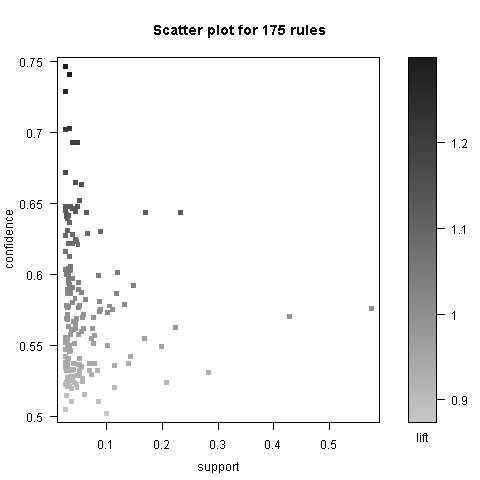
\includegraphics[width=90mm]{arulesviz.png}
\caption{Gráfico de dispersión de reglas generadas}
\label{arulesviz}
\end{figure}

Al correr Apriori con un minsup del 10\%, para ver cuales son estas reglas tan
fuertes respecto de las demás, se observan que son reglas cuyo lado izquierdo
esta vacío, o reglas tan triviales como \{sexo$=$hombre\} $=$$>$ \{rating$=$high\}

Es por esto que, para el análisis de películas realizado en este informe, se han
realizado, en primera instancia, 
 corridas de Apriori con soportes mínimos en el rango de \[0,009 ; 0,03\]
y confianza en el rango de \[0,05 ; 0,1\]

\section{Análisis}
En esta sección se analizan las mejores reglas generadas. 
Se muestran reglas que representan gustos
de películas, se intenta establecer reglas relacionadas con la
posición demográfica, como también analizar cambios y tendencias 
en los usuarios que califican películas.

\subsection{Reglas generales}
La primera impresión al ver las reglas generadas por Apriori, es que todas 
referencian a ratings positivos, siendo muy pocas las relacionadas con 
calificaciones mediocres o bajas. Es por esto que se analiza la frecuencia
de estas 3 calificaciones en la tabla \ref{rating_freq}, donde puede
claramente notarse que existe una tendencia a calificar las 
películas de forma elevada.

\begin{table}[ht!]
\caption{Frecuencia de ratings}
\label{rating_freq}
\centering
\begin{tabular}{l c}
Calificación & Frecuencia \\
low &  16\% \\
medium & 26\% \\
high & 58\%
\end{tabular}
\end{table}

\subsubsection{Directores mejor ranqueados}
La tabla \ref{table_best_directors} muesta las reglas relativas a los 
directores de películas mejor ranqueados.
\begin{table}[ht!]
\caption{Reglas relativas a directores}
\label{table_best_directors}
\centering
\begin{tabular}{l l l l }
regla & sop. & conf. & lift \\
\{Steven Spielberg\} $=$$>$ \{high\} & 2,36\% & 90\% & 1,15 \\
\{Alfred Hitchcock\} $=$$>$ \{high\} & 1,23\% & 95\% & 1,22 \\
\{James Cameron\} $=$$>$ \{high\} & 1,20\% & 89\% & 1,14 \\
\{Rob Reiner\} $=$$>$ \{high\} & 1,17\% & 92\% & 1,18
\end{tabular}
\end{table}

El soporte del director mejor ranqueado, Steven Spielberg, es de un 2,36\%. Aunque a nivel
porcentual este soporte parece bajo, a nivel nominal significa que de 888.500 ratings
totales, en 21.000 aparecen Steven Spielberg y de esas 18.900 la calificaron como un
rating \{high\}. Los soportes de la tabla \ref{table_best_directors} 
son nominalmente significativo. 

\subsubsection{Actores mejor ranqueados}
La tabla \ref{table_best_cast}   muestra las reglas relativas a los actores 
mejor ranqueados.
\begin{table}[ht!]
\caption{Reglas relativas a actores individuales}
\label{table_best_cast}
\centering
\begin{tabular}{l l l l }
regla & sop. & conf. & lift \\
\{Harrison Ford\} $=$$>$ \{high\} & 2,85\% & 91\% & 1,17 \\
\{Tom Hanks\} $=$$>$ \{high\} & 1,96\% & 89\% & 1,15 \\
\{Robert De Niro\} $=$$>$ \{high\} & 1,53\% & 87\% & 1,11 \\
\{Sean Connery\} $=$$>$ \{high\} & 1,35\% & 85\% & 1,09 \\
\{Arnold Schwarzenegger\} $=$$>$ \{high\} & 1,17\% & 77\% & 0,99
\end{tabular}
\end{table}


\subsubsection{dupla de actores mejor ranqueados}
La tabla \ref{table_best_tuple}   muestra las reglas relativas a la 
dupla de  actores mejor ranqueados.
\begin{table}[ht!]
\caption{Reglas relativas a dupla de actores}
\label{table_best_tuple}
\centering
\begin{tabular}{l l l l }
regla & sop. & conf. & lift \\
\{Carrie Fisher, Harrison Ford\} $=$$>$ \{high\} & 1,10\% & 95\% & 1,22 \\
\{Harrison Ford, Mark Hamill\} $=$$>$ \{high\} & 1,10\% & 95\% & 1,22 \\
\{Billy Dee Williams, Carrie Fisher\} $=$$>$ \{high\} & 0,70\% & 94\% & 1,20 \\
\end{tabular}
\end{table}

Esta tabla confirma aún mas que Harrison Ford es uno de los actores preferidos.

\subsubsection{Géneros}
La tabla \ref{table_genre} muestra los géneros mejores ranqueados.
\begin{table}[ht!]
\caption{Reglas relativas a actores individuales}
\label{table_genre}
\centering
\begin{tabular}{l l l l }
regla & sop. & conf. & lift \\
\{Drama\} $=$$>$ \{high\} & 23\% & 64\% & 1,11 \\
\{Comedy\} $=$$>$ \{high\} & 20\% & 54\% & 0,95 \\
\{Action\} $=$$>$ \{high\} & 14\% & 53\% & 0,93 \\
\{Romance\} $=$$>$ \{high\} & 9\% & 57\% & 0,99 \\
\end{tabular}
\end{table}

La base de datos contiene 18 categorías. En caso de que haya independencia en 
los gustos de géneros, el soporte de cada categoría debería tender a 5,55\%. 
Estos niveles de soporte, superiores al 10\% y algunos cercanos al 20\%,
implican que hay una preferencia sobre los géneros de drama, comedia,
acción y romance.

\subsubsection{A los hombres les gusta las peliculas de guerra}
La tabla \ref{table_male_ware} muestra que a los hombres
les gusta las películas de guerra, con o sin drama. Sin embargo,
hay una sensible preferencia por las películas de guerra 
pura, sin hechos dramáticos.

\begin{table}[ht!]
\caption{Reglas relacionadas con películas de guerra}
\label{table_male_ware}
\centering
\begin{tabular}{l l l l }
regla & sop. & conf. & lift \\
\{male, war\} $=$$>$ \{high\} & 3,75\% & 69\% & 1,20 \\
\{Drama, male, war\} $=$$>$ \{high\} & 2,51\% & 75\% & 1,29 \\
\end{tabular}
\end{table}

\subsubsection{El declive de la década de los ' 90}
Se han generado pocas reglas con calificaciones negativas. Una de las
que llama la atención es que muchas de ellas son relacionadas con películas
de la década de los ' 90, tal como muestra en la tabla \ref{table_year_90}.
\begin{table}[ht!]
\caption{El declive de los ' 90}
\label{table_year_90}
\centering
\begin{tabular}{l l l l }
regla & sop. & conf. & lift \\
\{25$-$34, low, male\} $=$$>$ \{1990\} & 3,44\% & 64\% & 1,20 \\
\{Comedy, low, male\} $=$$>$ \{1990\} & 3,07\% & 65\% & 1,21 \\
\{Drama, low\} $=$$>$ \{1990\} & 2,77\% & 67\% & 1,21 \\
\{Action, low, male\} $=$$>$ \{1990\} & 2,74\% & 66\% & 1,25 
\end{tabular}
\end{table}

\subsubsection{Las personas de 45 a 55, son quienes mejores califican}
La tabla \ref{table_age} muestra las reglas de las edades de los que
mejor califican. Probablemente no sea casualidad que ambas categorías 
son consecutivas.
\begin{table}[ht!]
\caption{Mejores calificaciones según la edad}
\label{table_age}
\centering
\begin{tabular}{l l l l }
regla & sop. & conf. & lift \\
\{45$-$49\} $=$$>$ \{high\} & 4,50\% & 62\% & 1,08 \\
\{50$-$55\} $=$$>$ \{high\} & 4,49\% & 59\% & 1,03 \\
\end{tabular}
\end{table}

\subsubsection{Géneros en común}
La tabla \ref{table_common_genre} muestra géneros relacionados 
entre si. 
\begin{table}[ht!]
\caption{Géneros en común}
\label{table_common_genre}
\centering
\begin{tabular}{l l l l }
regla & sop. & conf. & lift \\
\{Action,high,Sci-Fi\} $=$$>$ \{Adventure\} & 2,53\% & 51\% & 3,80 \\
\{high,Sci-Fi,Thriller\} $=$$>$ \{Action\} & 1,93\% & 76\% & 2,94 
\end{tabular}
\end{table}





\subsection{Reglas demográficas}
En esta sección se analiza las relaciones y preferencias según las variables 
demográficas estado y ciudad. 

\subsubsection{Estados y peliculas}
La tabla \ref{table_state_population} hace una comparación entre que porcentaje
de votos hicieron los estados que más calificaron y el porcentaje de habitantes
que tiene el estado respecto del total del país.

\begin{table}[ht!]
\caption{Votos y porcentaje poblacional}
\label{table_state_population}
\centering
\begin{tabular}{l l l}
estado & \% votos & \%población  \\
\hline
California & 18,07 & 11,78 \\
New York & 7,08 & 6,13 \\
Minnesota & 6,45 & 1,70 \\
Illinois & 5,50 & 4,07 \\
Texas & 5,23 & 8,36
\end{tabular}
\end{table}

Estos resultados muestran, principalmente, que tanto el estado de California
como el de Minesotta, son outlayers. Mientras que la población de
Minesota es del 1,70\% de la población de USA, el 6,45\% de los votos pertenecen
a este estado. El ratio es cercano a 4, lo que demuestra
que el estado de Minnesota tiene una preferencia a entretenerse viendo películas.
Algo similar sucede con el estado de California, donde su población es de casi el
12\% de los Estados Unidos, pero el 18\% de los votos totales pertenecen a este
estado. California también es un outlayer, pero este se comprende mas ya que la
mayor industria cinematográfica de Estados Unidos es Hollywood, que se encuentra
en el estado de California.

Otro de los puntos destacados que muestra la tabla \ref{table_state_population} es
que el estado de Texas no es propenso a entretenerse mirando películas, ya que los
votos de ese estado son menores en proporción, que la cantidad de habitantes.

Otra regla interesante es que el estado que mejor califica películas es California.

\begin{table}[ht!]
\centering
\begin{tabular}{l l l l }
regla & sop. & conf. & lift \\
\{high\} $=$$>$ \{CA\} & 10,44\% & 57\% & 1,03 \\
\{MN\} $=$$>$ \{HIGH\} & 3,81\% & 59\% & 1,03 
\end{tabular}
\end{table}

Este sesgo posiblemente también se deba a que Hollywood pertenece a California,
y mucha gente que vive de esta industria o se ve influenciada por su cercanía
física, 
esta calificando de forma positiva las películas. Es consistente que la regla
\{MN\} $=$$>$ \{HIGH\} tiene un soporte del 3,81\%, respecto del 10,44\% de 
California, ya que Minesotta no se encuentra influenciada por Hollywood.

\subsubsection{ciudades y peliculas}
La tabla \ref{citi_votes} muestra las ciudades que más votos realizaron y
la tabla \ref{citi_high} muestra las reglas de ciudades con mas calificaciones
positivas. Ambas tablas son consistentes entre si, y también son consistentes
con el análisis de los estados. Lo que llama la atención es que la ciudad de Los
Angeles, la 2\sptext{da} ciudad mas  pobladas de los Estados Unidos, 
ciudad que también pertenece al estado de California, 
\textbf{no} esta incluida entre las que mas votan\footnote{Los Angeles tiene
un 1\% de los votos totales}, como tampoco se pudieron generar reglas que 
incluyan a esta ciudad y a alguna calificación. Esta inexistencia
de reglas para esta ciudad particular, implicaría una ``meta-regla'' que
refleja que a la ciudad de Los Angeles \textbf{no} le gusta ver películas.
 
\begin{table}[ht!]
\caption{Votos por ciudades}
\label{citi_votes}
\centering
\begin{tabular}{l l }
ciudad & \% votos \% \\
Minneapolis & 2,52\% \\
New York & 2,37\% \\
San Francisco & 2,12\% \\
Saint Paul & 2,09\%  \\
\end{tabular}
\end{table}

\begin{table}[ht!]
\caption{Votos positivos por ciudad}
\label{citi_high}
\centering
\begin{tabular}{l l l l }
regla & sop. & conf. & lift \\
\{Minneapolis\} $=$$>$ \{high\} & 1,48\% & 58\% & 1,02 \\
\{New York\} $=$$>$ \{high\} & 1,38\% & 58\% & 1,01 \\
\{San Francisco\} $=$$>$ \{high\} & 1,22\% & 57\% & 0,99 \\
\end{tabular}
\end{table}


\subsubsection{Estados y géneros}
En esta sección se analiza la relaciones existentes entre estados y géneros
de películas. La tabla \ref{table_genre_state} resume la reglas mas relevantes al respecto.

\begin{table}[ht!]
\caption{Reglas mas relevantes sobre géneros y estados}
\label{table_genre_state}
\centering
\begin{tabular}{l l l l l }
nro & regla & sop. & conf. & lift \\
\hline
I & \{\} $=$$>$ \{Drama\} & 36\% & 36\% & 1 \\
II & \{\} $=$$>$ \{Comedy\} & 35\% & 36\% & 1 \\
III & \{\} $=$$>$ \{Action\} & 26\% & 26\% & 1 \\
IV & \{\} $=$$>$ \{Thriller\} & 19\% & 19\% & 1 \\
V & \{CA\} $=$$>$ \{Drama\} & 6,69\% & 37\% & 1,02 \\
VI & \{CA\} $=$$>$ \{Comedy\} & 6,32\% & 34\% & 0,97 \\
VII & \{CA\} $=$$>$ \{Action\} & 4,70\% & 26\% & 1,00 \\
VIII & \{CA\} $=$$>$ \{Thriller\} & 3,48\% & 19\% & 1,14 \\
IX & \{CA,high\} $=$$>$ \{Drama\} & 4,31\% & 41\% & 1,42 \\
X & \{CA,high\} $=$$>$ \{Comedy\} & 3,53\% & 33\% & 0,94 \\
\end{tabular}
\end{table}

La 1\sptext{er} a 4\sptext{ta} regla muestra que en todo Estados Unidos, 
la gente mira príncipalmente pelícuas de drama y comedia, 
en 3\sptext{er} medida de acción y en 4\sptext{ta}  Thriller\footnote{
Tener en cuenta que una película puede tener más de 1 género}. 
La 4\sptext{ta} a 8\sptext{va} regla se muestran las asociaciones mas fuertes que del 
lado izquierdo pertenece a un estado, y del derecho a un género
de película. Las 4 reglas tienen un soporte relativamente significativo y
pertenecen todas al mismo estado: California, estado con mayores votaciones.
Lo más interesante, es que los géneros de películas más vistos en California,
coinciden con los de todo Estados Unidos, tanto en orden, como en distancia
relativa entre cada uno de ellos.
La 9ena y 10ma regla muestra las asociaciones con mayores soporte y confianza, cuyo
lado izquierdo tiene un estado y una calificación elevada, y el lado derecho
un género. Los resultados, no por casualidad, coinciden con las películas
mas vistas en California, como en todo Estados Unidos.

El análisis de la tabla \ref{table_genre_state} permite inducir que
California es un estado dominante en cuestión de género de peliculas. 

Sería interesante analizar si esta misma posición dominante se repite en el pasado.
Si llegase a ser así, pero con diferentes géneros, se podría pensar que la industria
cinematográfica de Holliwood sigue los gustos de California, y un cambio en los 
gustos de ese estado, impactaría en el tipo de películas que Estados Unidos produciría.

La tabla \ref{table_genre_state_high} muestra las reglas de asociaciones mas fuerte que
destacan los géneros mejores calificados para cada estado relevante.

\begin{table}[ht!]
\caption{Generos mejores calificados por estado}
\label{table_genre_state_high}
\centering
\begin{tabular}{l l l l }
regla & sop. & conf. & lift \\
\hline
\{CA,Drama\} $=$$>$ \{high\} & 4,31\% & 64\% & 1,11 \\
\{CA,Comedy\} $=$$>$ \{high\} & 3,53\% & 56\% & 0,97 \\
\{Drama,NY\} $=$$>$ \{high\} & 1,79\% & 63\% &  1,13 \\
\{Comedy,NY\} $=$$>$ \{high\} & 1,36\% & 54\% &  0,98 \\
\{Drama,MN\} $=$$>$ \{high\} & 1,50\% & 65\% &  1,07 \\
\{Comedy,MN\} $=$$>$ \{high\} & 1,37\% & 56\% &  0,88 \\
\{Drama,IL\} $=$$>$ \{high\} & 1,21\% & 61\% & 1,13 \\
\{Comedy,IL\} $=$$>$ \{high\} & 1,01\% & 50\% & 0,98 \\
\{Drama,TX\} $=$$>$ \{high\} & 1,22\% & 65\% & 1,15 \\
\{Comedy,TX\} $=$$>$ \{high\} & 1,11\% & 56\% & 0,98 \\
\{Drama,MA\} $=$$>$ \{high\} & 1,12\% & 66\% & 1,15 \\
\{Comedy,MA\} $=$$>$ \{high\} & 1,00\% & 58\% & 1,02 \\
\end{tabular}
\end{table}

Esta tabla refuerza aún más la posición dominante que tiene California sobre la industria
cinematográfica. En todos los estados mas destacados, los géneros de 
las peliculas mas vistas coinciden con los de California. La diferencia es el nivel de
soporte de estas reglas respecto a porcentaje poblacional e inclusive al porcentaje de
votos en esta encuesta. California tiene porcentajes relativos mucho mas fuertes, avalando
la hipótesis de que Hollywood produce películas del agrado de California, y el resto de
los estados mira las películas realizadas por su mayor productor.


\subsubsection{Ciudades y géneros}
Al intentar encontrar la existencia de relaciones entre ciudades y géneros, se
han encontrado las reglas de la tabla \ref{citi_genre}.

\begin{table}[ht!]
\caption{Generos mas vistos por ciudad}
\label{citi_genre}
\centering
\begin{tabular}{l l l l }
regla & sop. & conf. & lift \\
\{New York\} $=$$>$ \{Drama\} & 0,99\% & 42\% & 1,63 \\
\{Minneapolis\} $=$$>$ \{Drama\} & 0,93\% & 37\% & 1,02 \\
\{Seattle\} $=$$>$ \{High\} & 1,12\% & 63\% & 1,10 \\
\end{tabular}
\end{table}

Estas reglas no aportan información relevante, solo refuerzan el desarrollo
previo. Posiblemente la imposibilidad de encontrar una fuerte relación entre
ciudades y géneros se debe a 2 motivos:
\begin{itemize}
\item El nivel de granularidad de agrupamiento por ciudad es elevado.
\item Los géneros de películas mas vistas están muy concentrados. Los 3 géneros
mas importantes se llevan más del 70\% de la torta, haciendo insignificante la
producción de otros géneros. Si los géneros producidos estuviesen
distribuidos más uniformemente, 
posiblemente pueda esperarse que a la ciudad de Utah tenga preferencias por las
películas religiosas, los de New York por musicales y Las Vegas por películas 
para adultos.
\end{itemize}




\subsubsection{Análisis de usuarios}
En esta sección se analiza las características de los usuarios que realizan
calificaciones. Con este propósito se divide el set de datos en 3 grupos:
\begin{enumerate}
\item Los usuarios que calificaron películas en el año 2000.
\item Los usuarios que calificaron películas en el año 2001.
\item Los usuarios que calificaron películas desde el 2002 para adelante.
\end{enumerate}
El objetivo es encontrar características similares de los primeros 2 grupos
y verificar si éstas también se encuentran presentes en el último.

Para este análisis lo que primero se tiene en cuenta es la distribución
de la cantidad de votos de cada grupo.
\begin{tikzpicture}
  \pie{90/año 2000, 7/año 2001, 3/$>$$=$2002}
\end{tikzpicture}

El segundo paso a realizar es hacer algunas corridas exploratorias en cada
grupo y graficar la nube de puntos con el soporte de arulesViz. 

\begin{figure}[ht!]
\minipage{0.32\textwidth}
  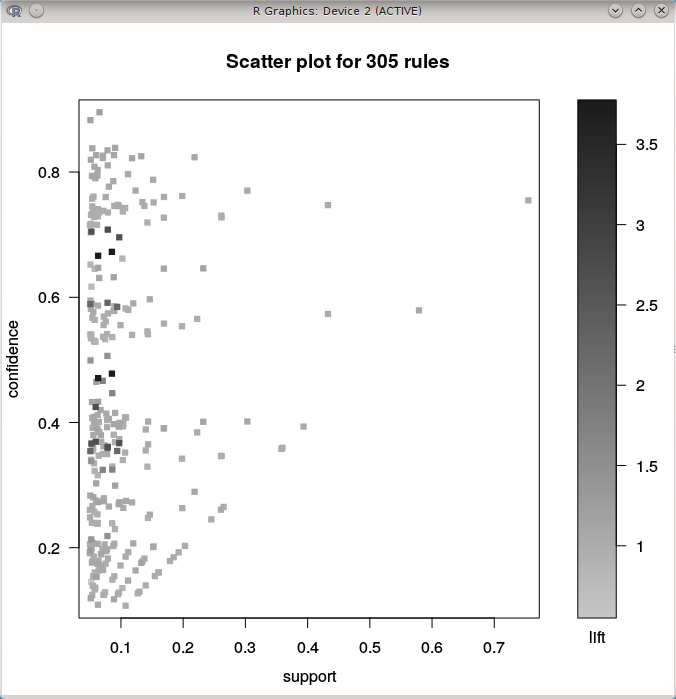
\includegraphics[width=\linewidth]{2000.png}
  \caption{Reglas para el año 2000. Minsup$=$0.05 Minconf$=$0.1}\label{fig:arules2000}
\endminipage\hfill
\minipage{0.32\textwidth}
  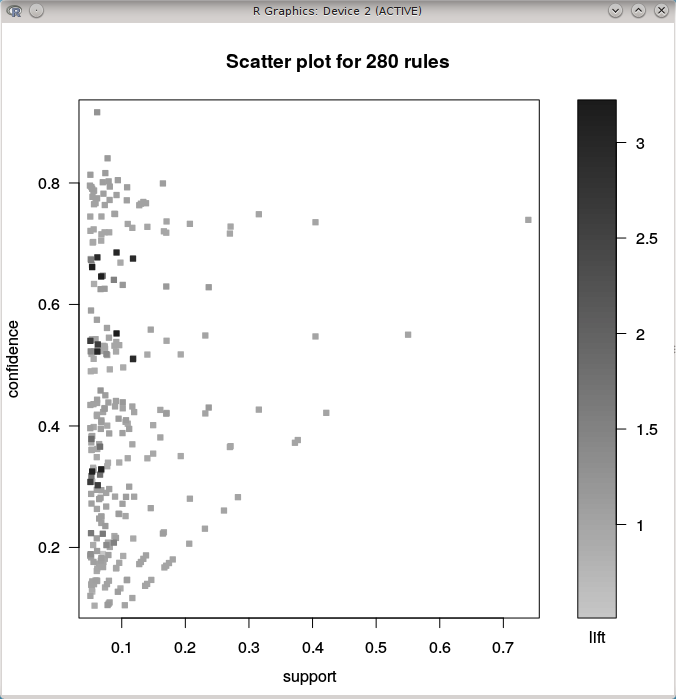
\includegraphics[width=\linewidth]{2001.png}
  \caption{Reglas para el año 2001. Minsup$=$0.05 Minconf$=$0.1}\label{fig:arules2001}
\endminipage\hfill
\minipage{0.32\textwidth}%
  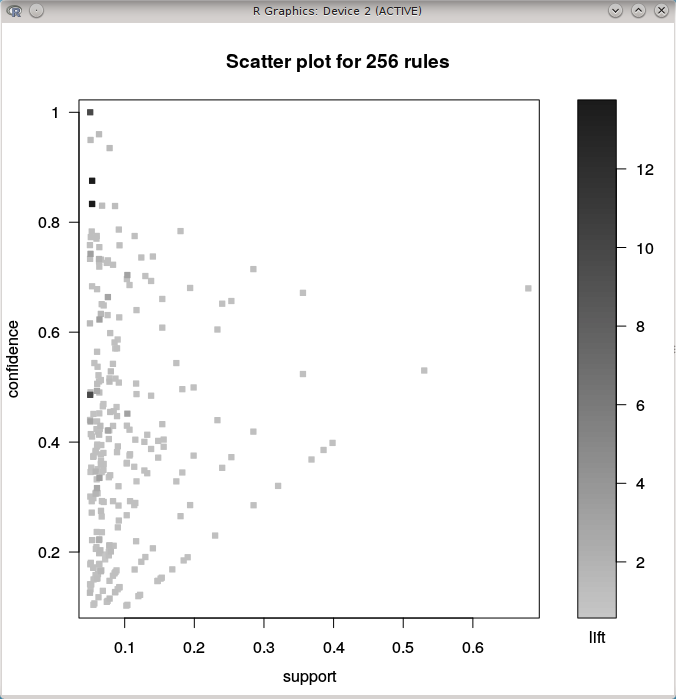
\includegraphics[width=\linewidth]{2002.png}
  \caption{Reglas para el año 2002 en adelante. Minsup$=$0.05 Minconf$=$0.1}\label{fig:arules2002}
\endminipage
\end{figure}

En las figuras \ref{fig:arules2000}, \ref{fig:arules2001} y \ref{fig:arules2002} 
se puede ver que, con los mismos parámetros, la cantidad de reglas
generadas son del mismo orden, como también, la distribución de las reglas
en la nube de puntos son muy similares en los 3 grupos.

Al navegar detenidamente la reglas más importantes de los 3 grupos 
se puede apreciar la semejanza
entre ellas. La tabla \ref{comparacion} muestra un resumen de éstas.

\begin{table*}[ht!]
\caption{Reglas de semejanza de usuarios}
\label{comparacion}
\centering
\begin{tabular}{|l l ||l l|l l|l l|}
	\hline
	nro & regla & 
	\multicolumn{2}{c|}{año 2000} & 
	\multicolumn{2}{c|}{año 2001} & 
	\multicolumn{2}{c|}{año 2002} \\
	     &  & sop & conf & sop & conf & sop & conf \\
	\hline
	I    & \{\} $=$$>$ \{male\} & 75\% & 75\% & 74\% & 74\% & 67\% & 67\% \\
	II   & \{\} $=$$>$ \{female\} & 24\% & 24\% & 26\% & 26\% & 32\% & 32\% \\
	III  & \{\} $=$$>$ \{Administ.\} & 13\% & 13\% & 17\% & 17\% & 15\% & 15\% \\
	IV   & \{\} $=$$>$ \{25$-$34\} & 39\% & 39\% & 42\% & 42\% & 40\% & 40\% \\
	V    & \{\} $=$$>$ \{35$-$44\} & 20\% & 20\% & 17\% & 17\% & 14\% & 14\% \\
	VI   & \{\} $=$$>$ \{18$-$24\} & 18\% & 18\% & 23\% & 23\% & 22\% & 22\% \\
	VII  & \{\} $=$$>$ \{high\} & 58\% & 58\% & 55\% & 55\% & 53\% & 53\% \\
	VIII & \{\} $=$$>$ \{medium\} & 26\% & 26\% & 28\% & 28\% & 28\% & 28\% \\
	IX   & \{\} $=$$>$ \{low\} & 16\% & 16\% & 16\% & 16\% & 18\% & 18\% \\
	X    & \{H. Ford\} $=$$>$ \{high\} & 2,18\% & 74\% & 1,33\% & 66\% & 1,25\% & 65\% \\
	XI  & \{18$-$24\} $=$$>$ \{Administ.\} & 8,54\% & 47\% & 11\% & 50\% & 10\% & 70\% \\
	XII & \{Advent\} $=$$>$ \{Action\} & 9,72\% & 69\% & 6,77\% & 64\% & 6,37\% & 62\% \\
	XIII  & \{romance\} $=$$>$ \{25$-$34\} & 6,05\% & 39\% & 6,09\% & 41\% & 6,06\% & 39\% \\
	XIV   & \{Administ.\} $=$$>$ \{high\} & 7,23\% & 56\% & 9,10\% & 52\% & 6,86\% & 46\% \\
	XV  & \{S. Spielberg\} $=$$>$ \{high\} & 1,81\% & 73\% & 1,10\% & 72\% & 1,07\% & 68\% \\
	\hline
\end{tabular}
\end{table*}

Las primeras 2 reglas muestran el sexo de los usuarios. 
En los 3 conjuntos de datos los hombres han tenido una posición mayoritaria holgada. 
Sin embargo, a partir del 2002, las mujeres tienen una
mayor participación en el set de votaciones, lo que se puede inferir 2 hipótesis
no excluyentes:
\begin{itemize}
\item La mujer esta teniendo mas partición en el rubro informático y/o acceso a Internet, ya que las 
votaciones se hacen on-line
\item Las mujeres están viendo mas películas a partir del año 2002.
\end{itemize}

Para obtener la tercer regla se solicita a R que devuelva la profesión que más votaciones 
ha realizado en cada set de datos, siendo los administrativos los primeros en todos los casos.
Dado que hay más de 20 profesiones, en caso de haber independencia de los gustos sobre profesiones, 
el valor esperado sería del 5\%, pero los administrativos tienen un valor comprendidos entre el
13 y 17\%, lo que comprueba que los administrativos son los más afines a entretenerse mirando
películas.

Luego se hace un análisis por edad. Al analizar este campo, se debe tener conciencia
sobre el entorno y sobre la posibilidad de acceso de las distintas edades al sistema de calificaciones.
Es posible que los chicos pequeño vean muchas películas, pero no tengan capacidad
de realizar votaciones. Del mismo modo, es posible que las personas muy adultas y
retiradas también sean asiduos expectadores, pero no tengan  interés en contribuir al sistema
de rating. Por lo tanto, hay que tomar conciencia que los análisis por edades pueden estar
sesgado por el interés de una generación en brindar información.

 La regla IV muestra
que el rango de 25 a 34 años es el que, por lejos, más peliculas mira. En todo momento
lleva una diferencia de aproximadamente el doble respecto al segundo.

Las reglas V y VI muestran que hay un cambio de tendencia con los rangos 35$-$44 y
18$-$24: A partir del 2001, el rango 18$-$24 tiene una participación más activa
al calificar películas que el de 35$-$44, ya que pasan de un 18\% en 2000, a
un 23\% y 22\% a partir del 2001.

Las reglas VII, VIII y IX muestran que tan bondadosos son los usuarios. En todo
momento los usuarios tienden a calificar positivamente las películas y muestran
rechazo por asignar calificaciones bajas. Las calificaciones positivas son 
constantemente más del doble de las mediocres y más del triple las negativas.
Sin  embargo, con el tiempo se va observando que el espectador se vuelve un
poco más exigente, ya que en el año 2000 los votos positivos son un 58\%, en
2001 un 55\% y desde el 2002 un 53\%.

Para generar la regla X se solicita el actor mejor calificado en cada dataset.
En todos estos Harrison Ford esta liderando el ranking. 

Para generar la regla XI, se pide a R que retorne las profesiones más relevantes
para cada rango de edad, siendo \{18$-$24\} $=$$>$ \{Administ.\} las de 
mayor soporte en todo momento.

La regla XII muestra que las personas que miran películas de aventuras, también
observan de acción. Esta regla se conserva en los 3 períodos analizados.

La regla XIII se analiza cual es el rango de edad preferido para las películas
románticas. En todos los set de datos fue el rango de 25$-$34, con un nivel
de soporte y confianza parejo en todo momento. Esto podría inducir que, 
por cuestiones psicológicas, los jovenes de 25 a 34 años son los más 
románticos.

Para generar la regla XIV se le pide al software que devuelva cual es la profesión
más generosa al calificar películas. Los administrativos son lideres en este
aspecto con el correr del tiempo.

Para la regla XV se pide el director de cine mejor calificado en cada período.
Steven Spielberg estuvo en la vanguardia en todo momento.

Por último, en la tabla \ref{genre_female} se analiza cual 
es el género mas visto por las mujeres en cada momento.

\begin{table}[ht!]
\caption{Generos mas escogidos por las mujeres}
\label{genre_female}
\centering
\begin{tabular}{l l l l }
year & regla & sop. & conf. \\
2000 & \{Romance\} $=$$>$ \{female\} & 5,22\% & 33\%  \\
2001 & \{Comedy\} $=$$>$ \{female\} & 10,12\% & 27\%  \\
$\geq 2002$ & \{Romance\} $=$$>$ \{female\} & 6,33\% & 41\%  \\
\end{tabular}
\end{table}

Tanto en el año 2000 como a partir del 2002, es el género romántico. Sin embargo, 
en el año 2001, el género de comedia prima por sobre el romance en más de 100\%:
en 2001 y desde 2002, el soporte de \{Romance\} $=$$>$ \{female\} es de entre
un 5 y 6\%, pero en 2001, la regla \{Comedy\} $=$$>$ \{female\} es de un 10\%.

Previo a finalizar esta sección, debe recordarse y tenerse en cuenta que 
 el 90\% de los datos que están en el dataset son del año 2000, quedando solo un 7\%
para el año 2001 y un 3\% para los años posteriores. Pese a que un  3\% 
no es un porcentaje significante, son 24.000 votaciones, número no despreciable.
Como se analizaron cada rango de tiempo en dataset independientes, el soporte
y la confianza de las reglas son comparables entre si, independientemente de la 
cantidad nominale de datos, ya que estos resultados son porcentuales.

\section{Conclusiones}
La primera conclusión que se puede obtener es que las reglas de asociaciones requiere
un trabajo arduo para preparar los datos. No se puede bajar los datos de una base de datos
y correrlos en Weka o R, como puede hacerse en un análisis de componentes 
principales, de correspondencia, de clasificación o de clustering. Se requiere limpiar 
datos, agrupar, discretizar y transformar, 
para generar los datasets deseados. Se debe generar rutinas que permitan generar nuevos
sets de datos de forma sencilla, cuestión de poder impregnarse en el problema fácilmente.

La segunda conclusión es que el algoritmo de Apriori implementado en la librería arules
es eficiente y puede correr más de 800.000 transacciones en cuestión de segundos. La principal
latencia de la librería es al cargar los datos, ya que los almacena pre-procesados.

La tercera conclusión es que no existe una única salida de Apriori, como si existe una única
regresión lineal. El usuario debe ir variando
los parámetros y ver las salidas generadas para identificar si hay reglas de asociaciones
triviales o interesantes. El usuario debe comparar las salidas de varios set de datos para
llegar a conclusiones que sean relevantes. Existen herramientas de visualización que simplifican
encontrar los parámetros de Apriori adecuados.

Por último, las reglas de asociaciones dan soporte para encontrar asociaciones
que son difícil de conocer tan solo con explorar la base de datos. Estas asociaciones tienen
que ser del tipo ``si sucede X, entonces sucede Y''. Se ve en el trabajo
como puede encontrarse relaciones entre edad y profesiones, géneros relacionados entre si,
cual es la edad con mayor atracción hacia los romances, y hasta se logra identificar
que el estado de California como el de Minnesota son outlayer. Esta información puede
ser utilizada para la toma de decisiones. Posiblemente, si un
fondo de inversión quiere construir un complejo de cines, Minnesota podría ser el 
lugar que sugieren las reglas de asociación.

\section{Posibles mejoras y consideraciones}

Un problema común cuando las personas juzgan, es la dificultad de otorgar una
calificación justa y uniforme para un mismo objecto. Algunos jueces pueden ser
mas bondadosos y otros más exigentes. Este inconveniente se ve a la perfección
en el problema de las películas, ya que más del 50 \% de los votos son positivos
y menos del 16\% son negativos. El sesgo de los calificadores es sumamente notable.
Este inconveniente puede salvarse normalizando las calificaciones, hecho que no
ha sido realizado en este análisis.

Crear estructuras de datos y objetos customs para el pre-procesamiento, puede
ser una solución adecuada cuando los requerimientos son claros y poco
volátiles. El pre-procesamiento de las reglas de asociación es muy dinámico. 
Muchas veces se realizan corridas de Apriori, se ven algunos inconvenientes,
y se busca generar nueva información, transformarla o filtrarla. En otras
palabras, el preprocesamiento y el procesamiento tienen un alto
nivel de acoplamiento. Cuando se
pretende generar nuevos datos, a veces modificar las estructuras de datos 
internas demanda tiempo o se pierde compatibilidad con versiones anteriores. Es
por esto que una vez finalizado el análisis, la experiencia muestra a los
autores que almacenar los datos en una base de datos puede agilizar
el desarrollo del preprocesamiento. No tiene que ser una base de datos
transaccional, concurrente, ni cliente-servidor. Un SQLite3 es suficiente
para generar estructuras de datos uniformes, accesibles desde el exterior
y con capacidad para filtrar, transformar y sumarizar información.

A su vez, la base de datos de grafos pueden resultar eficientes para representar
los datos y sus relaciones. Se considera conveniente hacer un análisis de 
reglas de asociaciones usando este tipo de motor de bases de datos.


\end{document}
